\input slide_preamble
\input preamble

\begin{document}

{\Huge


\centerline{\bf TTIC 31230, Fundamentals of Deep Learning}
\bigskip
\centerline{David McAllester, Autumn 2020}

\vfill
\centerline{\bf Learning Theory I}
\vfill
\centerline{\bf The Occam Generalization Guarantee}
\vfill
\centerline{\bf aka: The Free Lunch Theorem}
\vfill
\vfill

\slide{Chomsky vs. Kolmogorov and Hinton}

\includegraphics[width=1.0 in]{\images/Chomsky} \begin{minipage}[b]{8in} Noam Chomsky: 
Natural language grammar cannot be learned by a universal learning algorithm.
This position is supported by the ``no free lunch theorem''.\end{minipage}

\vfill
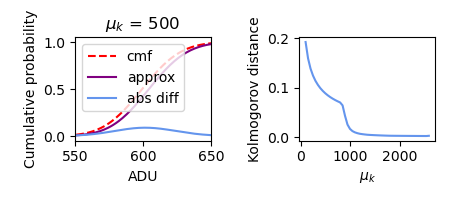
\includegraphics[height=1.0 in]{\images/Kolmogorov}
\includegraphics[height=1.0 in]{\images/Hinton}
\begin{minipage}[b]{7in}
Andrey Kolmogorov, Geoff Hinton: Universal learning algorithms exist. This position is supported by the ``free lunch theorem''.
\end{minipage}

\slide{The No Free Lunch Theorem}

\includegraphics[width=1.0 in]{\images/Chomsky} 

Without prior knowledge, such as universal grammar, it is impossible to make a prediction for an input you have not seen in the training data.


\vfill
{\bf Proof:} Select a predictor $h$ uniformly at random from all functions from ${\cal X}$ to ${\cal Y}$ and then take the data distribution to draw pairs $(x, h(x))$
where $x$ is drawn uniformly from ${\cal X}$.  No learning algorithm can predict $h(x)$ where $x$ does not occur in the training data.


\slide{The Occam Guarantee (Free Lunch Theorem)}

Consider a classifier $f$ written in C++ with an arbitrarily large standard library.

\vfill
Let $|f|$ be the number of bits needed to represent $f$.

\slide{The Occam Guarantee (Free Lunch Theorem)}

\vfill
$$0 \leq {\cal L}(h,x,y) \leq \lmax$$
\begin{eqnarray*}
{\cal L}(h)  & = &  E_{(x,y)\sim \mathrm{Pop}}\;{\cal L}(h,x,y) \\
\hat{{\cal L}}(h) & = & E_{(x,y)\sim \mathrm{Train}}\;{\cal L}(h,x,y)
\end{eqnarray*}

\vfill
Theorem: With probability at least $1-\delta$ over the draw of the training data the following holds simultaneously for all $f$.

{\color{red} $${\cal L}(f) \leq \frac{10}{9}\left(\hat{{\cal L}}(f) + \frac{5\lmax}{N_\mathrm{Train}}\left((\ln 2)|f| +\ln\frac{1}{\delta}\right)\right)$$}


\slide{Occam Guarantee (Probability Form)}

Code length is inter-convertable with with probability.

$$P(h) = 2^{-|h|}\;\;\;\mbox{or}\;\;\;|h| = - \log_2 P(h)$$

\vfill
Instead of fixing the language (e.g., C++ with a large library) we fix a prior $P(h)$.

\vfill
    {\bf Theorem:} With probability
    at least $1-\delta$ over the draw of training data the following holds simultaneously for all $h$.

\vfill
    $${\cal L}(h) \leq \frac{10}{9}\parens{\hat{\cal L}(h) + \frac{5 L_\mathrm{max}}{N_\mathrm{Train}}\parens{- \ln \delta P(h)}}$$

\slide{Occam vs. Bayes}

For {\color{red} ${\cal L}(h,x,y) = -\ln P_h(y|x) \leq L_{\mathrm{max}}$} we have

\vfill
\begin{eqnarray*}
\mbox{Occam:}\;\;\;\;\;{\cal L}(h) & \leq & \frac{10}{9}\parens{\hat{\cal L}(h) + \frac{5 L_\mathrm{max}}{N_\mathrm{Train}}\parens{- \ln \delta P(h)}} \\
\\
h^* & = & {\color{red} \argmin_h \hat{\cal L}(h) + \frac{5 L_\mathrm{max}}{N_\mathrm{Train}}\parens{- \ln P(h)}}
\end{eqnarray*}

\vfill
\begin{eqnarray*}
\mbox{Bayes:}\;\;\;\;\;\;h^* & = & \argmax_h P(h|\train) \\
\\
h^* & = & {\color{red} \argmin_h \hat{\cal L}(h) + \frac{1}{N_\mathrm{Train}}\parens{- \ln P(h)}}
\end{eqnarray*}

\slide{Proof}

Define
$$\epsilon(h) = \sqrt{\frac{2{\cal L}(h)\parens{-\ln \delta P(h)}}{\lmax N_\mathrm{Train}}}.$$

\vfill
By the relative Chernov bound we have

\vfill
$$P_{\mathrm{Train} \sim \mathrm{Pop}}\parens{\frac{\hat{{\cal L}}(h)}{\lmax} \leq \frac{{\cal L}(h)}{\lmax} - \epsilon(h)} \leq e^{-N_\mathrm{Train}\frac{\epsilon(h)^2\lmax}{2{\cal L}(h)}} = \delta P(h).$$

\slide{Proof}

$$P_{\mathrm{Train} \sim \mathrm{Pop}}\parens{\hat{{\cal L}}(h) \leq {\cal L}(h) - \lmax\epsilon(h)} \leq \delta P(h).$$

\vfill
$$P_{\mathrm{Train} \sim \mathrm{Pop}}\parens{\exists h\;\hat{{\cal L}}(h) \leq {\cal L}(h) - \lmax\epsilon(h)} \leq \sum_h \delta P(h) =\delta$$

\vfill
$$P_{\mathrm{Train} \sim \mathrm{Pop}}\parens{\forall h\;{\cal L}(h) \leq \hat{{\cal L}}(h) + \lmax\epsilon(h)} \geq 1- \delta$$

\slide{Proof}

$${\cal L}(h) \leq \widehat{{\cal L}}(h) + \lmax\sqrt{{\cal L}(h)\parens{\frac{2\lmax \parens{- \ln \delta P(h)}}{N_\mathrm{Train}}}}$$

using
$$\sqrt{ab} = \inf_{\lambda > 0}\;\frac{a}{2\lambda} + \frac{\lambda b}{2}$$
\vfill
we get
$${\cal L}(h) \leq \widehat{{\cal L}}(h) + \frac{{\cal L}(h)}{2\lambda} + \frac{\lambda\lmax\parens{- \ln \delta P(h)}}{N_\mathrm{Train}}$$

\slide{Proof}
$${\cal L}(h) \leq \widehat{{\cal L}}(h) + \frac{{\cal L}(h)}{2\lambda} + \frac{\lambda\lmax\parens{-\ln \delta P(h)}}{N_\mathrm{Train}}$$

\vfill
Solving for ${\cal L}(h)$ yields

\vfill
$${\cal L}(h) \leq \frac{1}{1-\frac{1}{2\lambda}}\parens{\hat{{\cal L}}(h) + \frac{\lambda\lmax}{N_\mathrm{Train}}\parens{-\ln\delta P(h)}}$$

\vfill
Setting $\lambda = 5$ brings the leading factor to 10/9 which seems sufficiently close to 1 that larger values of $\lambda$ need not be considered.

\slide{END}

}
\end{document}
